\documentclass[11pt,a4paper,oneside]{article}
\usepackage[utf8]{inputenc}
\usepackage{amsmath}
\usepackage{amsfonts}
\usepackage{amssymb}
\usepackage{graphicx}
\usepackage{color}
\usepackage {tikz}
\usetikzlibrary {er}
\usepackage[left=2.00cm, right=2.00cm, top=1.00cm]{geometry}
\graphicspath{{./}}

\begin{document}
	\title{DS 256 - Scalable Systems for Data Science \\ Assignment 0}
	\author{Shriram R. \\ M Tech (CDS) \\ 06-02-01-10-51-18-1-15763}
	\maketitle
	
	\section{Introduction}
	Analytics of Twitter data has been performed using Apache Spark through its Java interface. The experimental setup, results, plots and analysis are described in detail in the following sections.
     
    \section{Experimental Setup}
    
    \subsection{Hardware}
    Experiments were performed on a commodity cluster having 24 compute nodes. Each node has a 8-core AMD Opteron 3380 processor clocked at 2.6Ghz along with 32GB RAM and 2TB HDD and runs Ubuntu 16.04 LTS (64 bit) with Linux 4.4.0-139-generic. The nodes are connected through a Gigabit Ethernet switch.
    
    \subsection{HDFS and Spark}
    The HDFS environment has a capacity of 30.93TB with block size 128MB, replication factor of 2 and heartbeat delay of 3s. The global configuration of Spark for all experiments is 4 executors (containers) each having 4 cores and 8GB of memory. The Driver memory was set to 512MB. Apache YARN was used to coordinate the job execution and jobs were submitted through cluster mode. Experiment specific detail if any is provided below.
    
    \subsection{Dataset}
    The dataset used is a collection of 1\% of tweets sampled from Twitter between 17th Oct - 16th Dec 2016. The total dataset size is about 955GB and is stored in HDFS by partitioning the dataset into 3984 files of comparable size (approx. 300MB). Each tweet is described in Twitter Tweet JSON format and is of size approximately 5-10KB . The structure of JSON is described in [1].
  
    \section{Histogram}
    The pseudocode for the histogram of hashtags per tweet is given below,
    
    \begin{verbatim} 
          // Load text file into RDD
       1. JavaRDD twitterData = textFile(inputFile)
          // Parse JSON and get the hash count along with User ID
       2. JavaPairRDD hashCount = twitterData.flatMapToPair(getHashCount()) 
          // Get the average hashtag per tweet for each user
       3. JavaRDD avgPerUser = hashCount.reduceByKey(x, y -> x+y).map(sum/count)
          // Get the bucket values and frequencies for the given bucket count
       4. histogram = avgPerUser.histogram(bucketCount)
       5. Write histogram to HDFS     
    \end{verbatim}    
    The job was executed for the full dataset using the global configuration. The job took about 2.9 hours to complete. The job initially sustained failed stages which took about 4.5 hours. This occurred due to failure in metadata fetch. The job generated about 17.9GB of Shuffle data. The no. of partitions in the initial RDD is 9406. Bucket count was chosen arbitrarily as 20 and the result is plotted below,
    
    \begin{center}
    	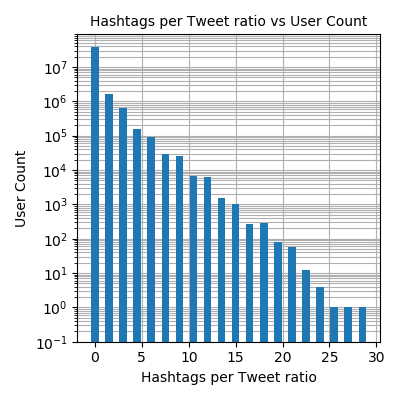
\includegraphics[scale=0.6]{1.png}		
    \end{center}

	It can be observed that the user count decreases as the Hashtag per tweet ratio increases. About 93.5\% of the users fall in the first bucket. The maximum Hashtag per tweet ratio in the given dataset is about 28.5 and the average value is about 0.16.
	
	\section{Co-occurring Hashtags}
	The pseudocode for finding the top 100 frequently co-occurring hashtags is given below,
	
	\begin{verbatim}
	       // Load text file into RDD
	    1. JavaRDD twitterData = textFile(inputFile)
	       // Parse JSON and get the hash tag pairs available in each tweet
	    2. JavaPairRDD hashTags = twitterData.flatMapToPair(getHashTags()) 
	       // Get the count for each distinct hash tag pair, sort descending by value
	    3. JavaRDD hashCount = hashTags.reduceByKey(x, y -> x+y).mapToPair(swap key-value)
	                                                            .sortByKey(false)
	       // Get top 100 frequent hash tag pairs
	    4. pairs = hashCount.take(100)
	    5. Write histogram to HDFS 
	\end{verbatim}
	
	The job was executed for the full dataset using the global configuration. The job took about 2.8 hours to complete and generated 9.4GB of Shuffle data. The no. of partitions in the initial RDD is 9406. The list of top 100 pairs of Hashtags along with their frequencies is available in [3]. The frequency of occurrence for these pairs is plotted below, 
	
	\begin{center}
		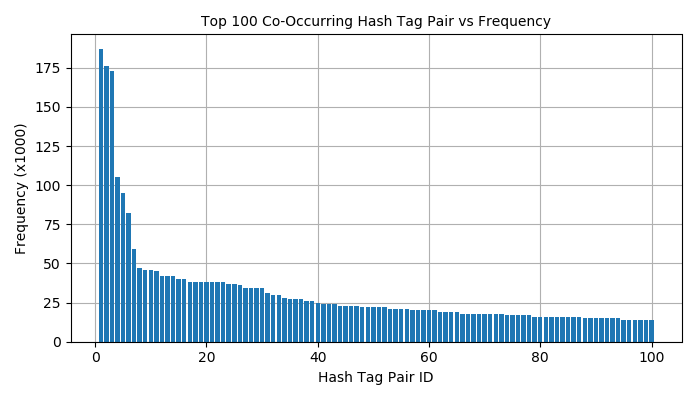
\includegraphics[scale=0.6]{2.png}		
	\end{center}

    The Hash Tag Pair IDs are alloted in the decreasing order of frequency. It can be observed that the frequency drops exponentially along the x-axis. The most frequent pair of Hash Tags was present in about 187,000 tweets. The Hash Tags were from different languages.
    
    \section{Temporal Interaction Graph}
    
    The pseudocode for getting the temporal interaction graph is given below,
    
    \begin{verbatim} 
       // Load text file into RDD and persist for reuse
    1. JavaRDD twitterData = textFile(inputFile).persist(StorageLevel.MEMORY_AND_DISK())
       // Parse JSON, get the vertex info and reduce to get
          the list of temporal properties for each vertex
    2. JavaRDD vertexInfo = twitterData.flatMapToPair(getVertex()).reduceByKey().map()
       // Parse JSON, get the edge info and reduce to get
          the list of temporal properties for each edge
    3. JavaRDD edgeIfo = twitterData.flatMapToPair(getEdge()).reduceByKey().map()
       // Save Vertex Info to HDFS as a single partition
    4. vertexInfo.coalesce(1, True).saveAsTextFile(vertexFile)
       // Save Edge Info to HDFS as a single partition
    5. edgeInfo.coalesce(1, True).saveAsTextFile(edgeFile)     
    \end{verbatim}
    
    The job was executed only on 1\% of the dataset. The job took a total of 9.1 minutes to complete and generated about 180MB of Shuffle data. The no. of partitions in the initial RDD is 111. Also, this experiment was run on a different setup having 8 containers, 4 cores per container and each having 16GB of memory. Execution on larger dataset sizes resulted in job failures due to insufficient memory and/or workers getting disconnected and in some cases few tasks that were running indefinitely. 
    
    The no. of vertices obtained is 2,217,705 and the no. of edges obtained is 1,238,318. The regular expression used to get the 1\% dataset files is tweets-10[0-3][0-9]*.txt 
    
    \section{Scaling Experiments}
    
    \emph{Hypothesis}: The FreqCount (Histogram) algorithm was used for these scaling experiments. The experiments studies the time taken to run the job with different dataset sizes for the same compute setup. The time taken for job completion has to linearly increase with the dataset size since the work done per Tweet is mostly constant. \\
    \emph{Setup}: The same global setup described in Section 2 was used for performing these experiments \\
    \emph{Input}: Different datasets comprising of 1\%, 5\%, 10\%, 15\% and 100\% of the total data  \\    
    The time taken for different dataset sizes is plotted as a Log-Log plot below,  
    
    \begin{center}
    	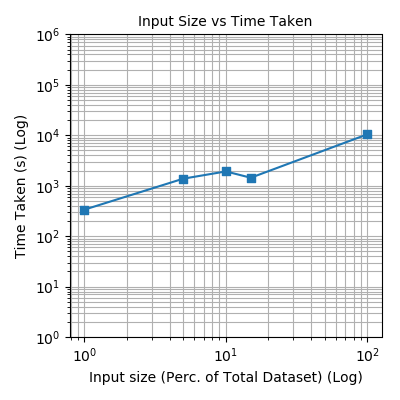
\includegraphics[scale=0.6]{3.png}		
    \end{center}    

    It can be observed that the time taken generally increases with the dataset size. However, there is a decrease in time for 15\% dataset size. This is due to different load conditions in the cluster present at the time of experiments. 15\% experiment was run at a time with lesser load than the other sizes. Also, note that the question asked for a 25\% dataset run but 15\% dataset was run instead by error. \\
    
    It can also be observed from the slope of line in the plot that there is a sub-linear (slope $<$ 1) relationship between size and time taken. 
    
    \section{Note}
    JSON parsing was done using json-simple library. All other operations/transformations were performed using in-built Spark and Java libraries.
        
    \section{References}
    \begin{list}{}{}
    	\item 1. https://developer.twitter.com/en/docs/tweets/data-dictionary/overview/tweet-object.html
    	\item 2. DS 221 Course lecture notes
    	\item 3. hdfs:///user/shriramr/output7.txt
    	\item 4. https://spark.apache.org/docs/latest/api/java/index.html
    	\item 5. https://www.geeksforgeeks.org/parse-json-java/
    \end{list}  
    
\end{document}